\section{Introduction}
\label{sec:intro}
%\gist{
  %Section gist: The era of reconfigurable architectures is here, as they achieve higher energy efficiency over general purpose processors in certain application domains.
  %FPGAs are successful, but fine-grained reconfigurability incurs hardware overheads, the biggest of all in the programmable interconnect.
  %CGRAs have been proposed to alleviate this problem by providing coarse-grained reconfigurable abstractions. This increases compute density,
  %but also makes the interconnect bulky and less flexible. Hence, a good interconnection network design is key to achieving a balanced
  %design for a coarse-grained architecture. \\
%
  %Static interconnects use statically programmable switches to reserve links between communicating
  %units for the lifetime of the application; great for bandwidth, but does not allow link sharing.
  %Static interconnects place immense burden on the compiler to produce a valid placement and routing for applications. Applications
  %that cannot be routed successfully can simply not execute, even though ample compute resources are available.
  %As a result, architectures with purely static interconnects end up overprovisioning the number of links to increase flexibility and path diversity, which adds considerable area
  %overhead. In addition, having such a flexible interconnect also increases the search space for the compiler, which increases compile times. \\
%
  %Dynamic interconnects allow sharing links between more than one pair of communicating units. Communication takes place at the granularity of individual packets, where
  %each packet contains some route metadata and a payload. Routers in the interconnect use various algorithms share to links between multiple competing senders, avoid deadlocks,
  %and ensure fairness. Dynamic networks offer greater flexibility and can simplify compilation. However, routers in dynamic networks often consume more area and power due to additional
  %buffers compared to a static switch. In addition, avoiding deadlocks in dynamic networks is a critical concern. \\
%
  %In this paper, we propose a hybrid interconnect that attempts to preserve the benefits of both static and dynamic interconnects. Specifically, we explore having a static interconnect
  %without overprovisioning, and use a second interconnect which is dynamic to spill over excess traffic. We describe our method to avoid deadlocks in the dynamic network. We also
  %describe our compiler infrastructure that allocates resources on the static and dynamic network. We evaluate our approach in detail on a broad range of benchmarks with different communication
  %patterns, which stresses the on-chip network by various amounts. \\
%
  %Key contributions: \\
%
  %Rest of the paper is organized as follows. Section 2 provides background. Section 3 dicusses our algorithm and compiler infrastructure. Section 4 provides a detailed evaluation.
  %Section 5 discusses related work. Section 6 concludes.
%}

%In recent years, industry and academia alike have shown increasing interest in 
Spatially reconfigurable architectures are programmable, energy efficient application accelerators offering the flexibility of software and the efficiency of hardware.
Architectures such as Field Programmable Gate Arrays (FPGAs) achieve energy efficiency by providing statically reconfigurable compute elements and on-chip memories in a bit-level programmable interconnect; this interconnect can be configured to implement arbitrary datapaths. FPGAs are used to deploy services commercially~\cite{microsoft, baidu, deephi}
and can be rented on the AWS F1 cloud~\cite{aws}. However, FPGAs suffer from overhead incurred by fine-grained reconfigurability; their long compile times
and relatively low compute density have hampered widespread adoption for several years~\cite{bolsens, calhoun, fpgaPower, fpgaSurvey}. 
Therefore, recent spatial architectures use
increasingly coarse-grained building blocks, such as ALUs, register files, and memory controllers, distributed in a programmable, word-level static interconnect.
Several of these Coarse-Grained Reconfigurable Arrays (CGRAs) have recently been proposed \cite{adres, kress, dyser, piperench, tartan, hrl, ti, hycube, plasticine}.

%Coarse Grained Reconfigurable Arrays (CGRAs) are a computing technology promising to combine a CPU's ease of programming, an FPGA's flexibility, and an ASIC's efficiency.
%CPUs suffer from a lack of compute resources: they only have a small number of computational units, and must use large memories for bookkeeping to support their programming model.
%ASICs allow the user to specify arbitrary circuits, and therefore can have more computing resources, but are limited by high costs and long design times.
%FPGAs provide fast reconfigurability, but pay a heavy price: a large portion of every FPGA is devoted to routing resources, and synthesis tools struggle with the massive graphs necessary to account for bit-level resources.
%CGRAs have a distributed set of processing elements and memories, which are traditionally connected using a word-level static interconnect.
%In Plasticine, the CGRA we target for this work, the processing elements are 16 lane, 6 stage SIMD pipelines and the memories are 256kiB SRAMs; the interconnect is composed of 32b and 512b links.
%Because the network resources themselves are wider, a good interconnection network design is key to achieving a balanced design.
Applications are mapped to CGRAs by distributing computations spatially across multiple processing blocks and executing them in a pipelined, data-driven fashion.
%Compared with processor-based architectures, pipelining introduces fundamentally different communication patterns.
On traditional Networks on Chip (NoCs), communication is the result of explicit message passing by parallel workers or cache misses; these are bursty and relatively infrequent.
On CGRAs, however, applications are distributed by parallelizing and pipelining; pipelining introduces frequent and throughput-sensitive communication.
Because different applications are parallelized and pipelined differently, they have different communication requirements.
%Obtaining high performance requires maximizing on-chip resource utilization to exploit parallelism and data locality.
%TODO START HERE @acrucker
%Different applications exhibit different amounts of parallelism and pipelining; this translates to different communication requirements.

CGRAs need the right amount of interconnect flexibility to achieve high resource utilization; an inflexible interconnect constrains the space of
valid application mappings and hinders resource utilization. Furthermore, in the quest to increase compute density, CGRA data paths now 
contain increasingly coarse-grained processing blocks such as pipelined, vectorized functional units~\cite{plasticine, piperench, xilinx-acap}.
These data paths typically have a vector width of 8--16x~\cite{plasticine}, which necessitates coarser communication and higher on-chip interconnect bandwidth to avoid
creating performance bottlenecks. 
Although many hardware accelerators with large, vectorized data paths have fixed local networks~\cite{brainwave}, there is a need for more
flexible global networks to adapt to future applications.
Consequently, interconnect design for these CGRAs involves achieving a balance between the often conflicting requirements of high bandwidth and high flexibility.

Interconnects can be classified into two broad categories: \emph{static} and \emph{dynamic.}
 {Static interconnects} use switches programmed at compile time to reserve high-bandwidth links between communicating units for the lifetime of the application.
%However, as links cannot be shared between multiple senders, flexibility in static interconnects is achieved by over-provisioning the number of links, which adds significant area overhead.
%In addition, static interconnects place an immense burden on the compiler to produce a successful application mapping and do not allow gracefully degrading
%performance; applications that cannot be placed and routed successfully cannot execute, even though ample compute resources are available. 
CGRAs traditionally employ static interconnects~\cite{cgraSurvey1, cgraSurvey2}.
%
In contrast, {dynamic interconnects}, or NoCs, contain routers that allow links to be shared between more than one pair of communicating units.
NoC communication is typically packet-switched, and routers use allocators to fairly share links between multiple competing packets.
%However, a dynamic network can support more links with the same area, making it a logical choice for infrequently used links.
Although static networks are fast, they require over-provisioning bandwidth and can be underutilized when a dedicated static link is reserved for a logical link that is not 100\% active. 
While dynamic networks allow link sharing, the area and energy cost to transmit one bit of data is higher for routers than for switches, making bandwidth scaling more expensive in dynamic networks than in static networks.
%Dynamic networks offer greater flexibility and allows more graceful performance degradation. However, congestion in dynamic networks causes bandwidth loss which adversely affects throughput.
%Routers also consume more area and power than a static switch due to additional logic and buffers. Tiled processor architectures and CMPs commonly use dynamic interconnects~\cite{ocn-cmp, ocn-synthesis}.

\begin{figure}
\centering
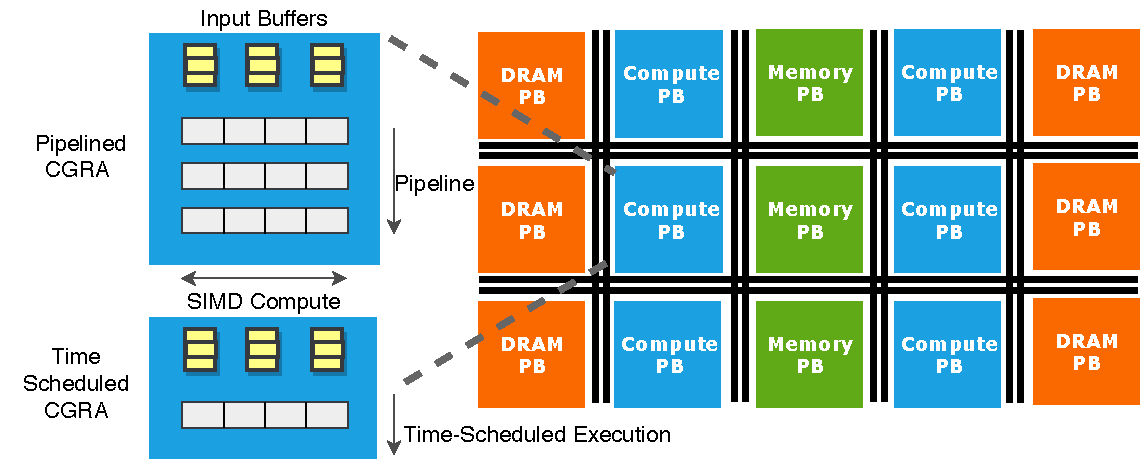
\includegraphics[width=1\columnwidth]{figs/arch1.pdf}
%\caption{Link activation count cumulative density function and averaged link activation rate
  %distribution (green: vector, pink: scalar). }\label{fig:link}
  \caption{Abstract machine model of our target CGRA, with compute, memory, and DRAM Physical Blocks (PBs).}\label{fig:arch}
\end{figure}

\if 0
Motivated by the need to combine the flexibility of a dynamic network with the bandwidth guarantees of a static network, tiled processors such as the academic Raw~\cite{raw} processor and
the commercial Tile~\cite{tile} processor use variants of the scalar operand network (SON)~\cite{son}. SONs are hybrid interconnects that combine a static and two dynamic networks to efficiently route scalar operands
between tiles. To support the bandwidth requirements of vectorized CGRAs, though, the network must use buses and flit widths to match vector widths of around 512 bits. Naively using a wider interface with the aforementioned SON faces several problems:
(i)   multiple physical networks may not be practical, as wires and routing tracks become a critical resource,
(ii)  the number of Virtual Channels (VCs) and buffer depth are more constrained as they cost significantly more area and power, and
(iii) message-dependent deadlocks~\cite{deadlock-tpds03} are possible as multiple independent data streams can share routers and a common end point, requiring a low-cost deadlock avoidance solution.

In this paper, we address the above challenges and propose a hybrid interconnect that attempts to preserve the benefits of both static and dynamic interconnects for vectorized CGRAs.
Using communication patterns from a diverse set of applications, we identify the space of interconnection networks with scalar and vector communication granularities and the
opportunities for dynamism. We then describe our compiler stack that maps the application
using a series of transformations to a vectorized CGRA with compute and memory blocks.
%We introduce a unique challenge in guaranteeing deadlock freedom with DOR, and describe our static VC allocation scheme that guarantees deadlock freedom.
%Next, we describe our static VC allocation scheme that guarantees deadlock freedom.
Next, we evaluate the performance, area, and power of several interconnection designs using ASIC synthesis of switches and routers with a 28nm industrial technology
and cycle-accurate simulations of the CGRA. Our evaluation results show that two bi-directional links per switch direction in the fully static interconnect
provide sufficient flexibility and bandwidth to place and route a diverse set of applications; the static network does not have to be significantly over-provisioned.
Finally, we also show that a hybrid network with an additional dynamic interconnect does not incur significant hardware overheads, thereby
providing a safety net against performance cliffs of unroutable designs on a fully static network.
\fi

In this paper, we start by detailing the key considerations involved in building a CGRA network, including those arising from network design, CGRA architecture, and the characteristics of spatially mapped applications.
Network designs must be carefully considered because vectorization magnifies inefficiencies: the increased network area of a vectorized design ensures that any overhead has a significant impact.
%although a small, scalar CGRA will not have much overhead, the increased network area of a vectorized design ensures that any overhead will have a significant impact on overall system cost.
%Network area scales superlinearly when moving from scalar to vector network due to increased wire capacitance in wide data-path.
Next, we evaluate the performance, area, and power requirements of several interconnection designs using cycle-accurate simulation and ASIC synthesis of a switch and router with a \SI{28}{nm} industrial technology library.
We then explore a variety of design points, including static, dynamic, and hybrid networks, decreased flit widths and VC counts for dynamic networks, and different flow-control strategies for static networks.

We show that CGRA network designs must consider application characteristics and the execution model of the underlying architecture.
Performance scales strongly with network bandwidth, with an 8x average performance gap between the best and worst configurations. 
The hybrid network gives the best network energy-efficiency: a 1.83x average improvement over the static network. On pipelined architectures,
hybrid networks can also match the performance per area of higher bandwidth, purely static networks with less than 8\% performance loss.
%Generally, pure static networks provide better performance per area with up to a 7x improvement, while hybrid networks with high static bandwidth and a small dynamic network as a safety net yield a 2.3x average energy efficiency improvement.
%Furthermore, we show that pipelined CGRAs perform better with a purely static, high-bandwidth network, whereas a time scheduled CGRA benefits from a hybrid network due to its lower bandwidth requirements.
%We also show that a hybrid network with an additional dynamic interconnect does not incur significant hardware overheads, thereby
%providing a safety net against performance cliffs of unroutable designs on a fully static network.
%Furthermore, we show that there are scaling limitations related to the size of the CGRA array: although the increased vector width decreases the control overhead and allows larger designs, the inherently planar organization limits the number of active nodes.
%We also show that a hybrid network with a dynamic interconnect and half the bisection bandwidth of the static network
%has a geomean performance loss of 1.27x, and an area overhead of 5.6\% relative to a fully static network, while providing a safety net against performance cliffs of unroutable designs on a fully static network.

The key contributions of this paper are:
\begin{enumerate}
    \item An analysis of key communication patterns exhibited by spatial architectures.
    \item A network-aware compiler flow that efficiently targets static, dynamic, and hybrid
      networks with varying granularities.
    %\item A technique to provision VCs for deadlock avoidance while minimizing area, and
    \item A quantitative analysis of the performance, area, and energy trade-offs involved in choosing a CGRA network, using benchmarks drawn from various application domains.
      %\item We determine that the best network for CGRAs is a hybrid network with vector static links, a specialized scalar network, and a dynamic network to ensure all routability.
\end{enumerate}

The rest of the paper is organized as follows:
Section~\ref{sec:back} provides background on the communication patterns that motivate interconnect design and describes the network design space explored in this paper.
Section~\ref{sec:method} describes our compiler flow for a vectorized CGRA, including how we physically map applications.
Section~\ref{sec:eval} details our evaluation methodology and experimental results.
Section~\ref{sec:related} discusses related work, and Section~\ref{sec:conclusion} offers concluding remarks.

%This interconnect is configured once, at compile time, to support all the possible data flows that the application may take; at runtime, crossbars are loaded with the configuration and valid/ready signals are used to coordinate the movement of data through these statically allocated links.
%Plasticine is an example of a CGRA that is specialized for computing on vector data---the processing elements (Pattern Compute Units, PCUs) are 16-lane, 6-stage SIMD arrays, and the memories (Pattern Memory Units, PMUs) are banked 16 ways and a total of \SI{256}{kiB} \cite{plasticine}.
%There are a total of 64 PCUs, 64 PMUs, and 4 DDR3 controllers in Plasticine, with a total area of \SI{113}{\mu m^2} and a clock rate of \SI{1}{GHz}.
%Instead of using solely a word-level interconnect, Plasticine also uses a vector interconnect that supports \SI{512}{b} per cycle.
%
%Dynamic networks are a promising alternative to static networks because they allow resources to be effectively shared at run time \cite{dally2001route}.
%Instead of assigning fixed resources to each network flow, routers throughout the chip arbitrate between packets, allowing an arbitrary number of logical routes to share the same set of physical links.
%This makes dynamic networks a promising technology for CGRAs: there is no longer an invisible ``cliff'' when placing applications, after which routing fails and the application must be refactored.
%Additionally, dynamic networks provide the possibility of using on-chip resources more efficiently, because multiple network flows may otherwise only use a small portion of their alloted time slots.
%
%However, packet-switched dynamic networks come with the possibility of large overheads to compensate for several common pathologies, including deadlock, poor allocation performance, and congestion.
%Deadlock occurs when packets wait on each other in a cycle, and is traditionally mitigated by restricting routing algorithms or using multiple Virtual Channels (VCs).
%However, restricting routing algorithms leads to the possibility of multiple routes attempting to use the same links, and can therefore cause congestion; muliple VCs increases buffering requirements.
%Poor allocation performance is compensated for by using speedup: making the router internals (crossbar, etc.) faster than the surrounding links---this can substantially increase the area and energy consumed by a router.
%Finally, adaptive and oblivious routing can send packets along varying routes, to alleviate congestion on any one link; this would require the addition of expensive reorder buffers at network endpoints and end-to-end flow control to track reorder buffer occupancy.
%
%In this paper, we propose a compiler-directed dynamic network for Plasticine, which is able to use high-level information about the program graph to statically optimize for a dynamic network.
%Our placer runs in seconds, and is able provide co-optimized solution to the placement, adaptive routing, and deadlock avoidance problems.
%The placer uses a derivative-free optimization technique and flexible heuristics to quickly explore a wide variety of configurations and can fix problems at multiple levels: for example, routing congestion can be alleviated by re-routing, re-placing, or reallocating VCs.

%\begin{outline}
%  \1 Discuss Plasticine I, and reiterate design parameters
%  \1 Discuss dynamic networks
%    \2 Show where the power goes by citing prior work---links/xbar/buffer
%    \2 Discuss why these are necessary (multiple VCs, etc.)
%  \1 Provide the qualitative rationale for dynamic networks (no cliff)
%    \2 Also discuss the yield/multitenancy implications
%  \1 Discuss the algorithms we used, with references to similar prior work
%    \2 We integrate placement/routing into a feedback loop, where problems with
%      one drive changes in the other
%    \2 We have a deadlock avoidance algorithm that uses the safe case for
%      guaranteed success
%    \2 Fast, guaranteed successful placement is a selling point
%  \1 Introduce the physical area/power methodology
%  \1 Introduce the set of baseline/alternate designs
%  \1 Summarize results and conclusions
%\end{outline}

